% Created 2024-09-25 Wed 00:53
% Intended LaTeX compiler: xelatex
\documentclass[letterpaper]{article}
\usepackage{graphicx}
\usepackage{longtable}
\usepackage{wrapfig}
\usepackage{rotating}
\usepackage[normalem]{ulem}
\usepackage{capt-of}
\usepackage{hyperref}
\usepackage{fontspec}
\usepackage{bookmark}
\setmainfont[Ligatures=TeX]{CMU Serif}
\usepackage{amssymb}
\usepackage{amsmath}
\setlength{\parindent}{0pt}
\author{Gleb Anohin}
\date{\today}
\title{analysis set}
\hypersetup{
 pdfauthor={Gleb Anohin},
 pdftitle={analysis set},
 pdfkeywords={},
 pdfsubject={},
 pdfcreator={Emacs 29.1 (Org mode 9.8)}, 
 pdflang={English}}
\begin{document}

\maketitle
\tableofcontents

\section{Множество}
\label{sec:org2b45d61}
\subsection{Определение}
\label{sec:orgadc730e}
Совокупность объектов (элементов) любой природы
\(\emptyset\) -- пустое множество, т.е. множество без элементов

\textbf{Каждый элемент множества входит в множество однократно, т.е. уникален}
\subsection{Обозначения}
\label{sec:org81070d8}
A, B, \ldots{}, M - множества
a, b, \ldots{}, m - обозначения элементов множества
\subsubsection{Задание множества}
\label{sec:org4c91b36}
\begin{enumerate}
\item Перечисление элементов \(M = \{1, 2, 3\}\)
\item С помощью характеристического свойства: \(A = \{x \in M: B(x)\}\)
B(x) - предикат, М - универсум
(Универсум -- базовое множество для рассматриваемой задачи)
\begin{enumerate}
\item \(M = N\)
\item \(A = \{x \in M: x \equiv 0 (mod 2) \}\)
\item \(A = \{x \in M: x \in A\}\) - тождественная запись
\end{enumerate}
\item \(M = \{\{\emptyset\}, \{\{\emptyset\}, \emptyset\}\}\)
\end{enumerate}

Множество A является подмножеством B если \(\forall b \in B \rightarrow b \in A\)
\(A \subset B\) или \(A \subseteq B\)
Собственное подмножество -- \(A \subsetneq B\)
\subsection{Мощность}
\label{sec:org39784f9}
Мощностью конечного множества \(A\) называется количество его элементов.
\(\# A = |A|\)

Множество \(A\) имеет счетную мощность, если существует биекция \(F: A \rightarrow N\)
\subsubsection{Экививалентность}
\label{sec:org8a71f8d}
\(A \textasciitilde B\) (равномощны), если биекция (взаимно-однозначное) существует \(F: A \rightarrow B\)
\subsubsection{Теорема Кантора}
\label{sec:org4d24072}
Обозначим \(2^A\) - множество всех подмножеств множества \(A\).

Множество всех пожмножеств множества \(A\) не эквивалентно \(A\).

Доказательство от противного:

Представим, что существует биекция \(F: 2^A \rightarrow A\).
Назовем элемент \(a \in A\) дефектным,
если \(a \notin M_a\), где \((M_a, a) \in F, M_a \subset A\) т.е. \(M_a \in 2^A\)

Назовем множество \(D = \{a \in A, a - \text{defect}\}\) дефектом.
Т.е. \(D \in 2^A, D \subset A\)

Рассмотрим \(d \in A: (D, d) \in F\).

Предположим, что \(d\) - дефектный, тогда \(d \in D\), но \(d \notin D\),
т.к. это заложено в определении \(F\).

В противном случае \(d\) - недефектный, но тогда он является дефектным, поскольку удовлетворяет \(d \notin D\).

Следовательно \((D, d) \notin F\)
\(\blacksquare\)
\subsection{Парадокс Рассела}
\label{sec:org462104c}
М - все
A - бреется сам
B - бреет бродобрей

\(A \cap B = \emptyset\)
\(A \cup B = M\)

Но бродобрей попадает в оба множества.
\subsection{Операции}
\label{sec:org965f022}
\subsubsection{Объединение}
\label{sec:orgd63e4d1}
\(A \cup B = \{x \in M: (x \in A) \land (x \in B)\}\)
\subsubsection{Пересечение}
\label{sec:orge751ba0}
\(A \cap B = \{x \in M: (x \in A) \lor (x \in B)\}\)
\subsubsection{Разность}
\label{sec:orgf6efddb}
\(A \ B = \{x \in M: (x \in A) \lor \neg{(x \in B)}\}\)
\subsubsection{Дополнение (типо до универсума)}
\label{sec:org56d265f}
\(\neg{A} = \{x \in M: \neg{(x \in A)}\}\)
\subsubsection{Симметрическая разность}
\label{sec:orge498a46}
\(A \triangle B = (A \cup B) \backslash (A \cap B)\)
\subsection{Законы}
\label{sec:orgbed5480}
Коммутативность (перестановочность)
\begin{enumerate}
\item \(A \cap B = B \cap A\)
\item \(A \cup B = B \cup A\)
\end{enumerate}
Аccоциативность (сочетательность)
\begin{enumerate}
\item \((A \cap B) \cap C = A \cap (B \cap C)\)
\item \((A \cup B) \cup C = A \cup (b \cup C)\)
\end{enumerate}
Дистрибутивность (распределенность)
\begin{enumerate}
\item \(A \cap (B \cup C) = (A \cap B) \cup (A \cap C)\)
\item \(A \cup (B \cap C) = (A \cup B) \cap (A \cup C)\)
\item \(A \backslash (B \cap C) = (A \backslash B) \cup (A \backslash C)\)
\item \(A \backslash (B \cup C) = (A \backslash B) \cup (A \backslash C)\)
\item \(\neg{A \cup B} = \neg{A} \cap \neg{B}\)
\item \(\neg{A \cap B} = \neg{A} \cup \neg{B}\)
\item \(A \cup \emptyset = A\)
\item \(A \cap \emptyset = \emptyset\)
\item \(A \cup U = U\)
\item \(A \cap U = A\)
\end{enumerate}
Идемпотентность
\begin{enumerate}
\item \(A \cup A = A\)
\item \(A \cap A = A\)
\end{enumerate}
Отрицание
\begin{enumerate}
\item \(\neg{\emptyset} = U\)
\item \(\neg{U} = \emptyset\)
\end{enumerate}
\section{Отображение}
\label{sec:org5b38f2a}
Пусть \(A, B\) - множества. Декартовым произведением называется
\(A \times B = \{(a, b): a \in A, b \in B\}\)

Отображением множества \(A\) на множество \(B\) - \(F \subset A \times B\).

Обозначение: \(F: A \rightarrow B\).
\subsection{Примеры}
\label{sec:org6716822}
\begin{enumerate}
\item \(A = N, B = N, F = \{(n, 1): n \in N\}\)
\item \(A = Z, B = N, F = \{(-1, m): m \in N\}\)
\item \(A = Z, B = N, F = \{(m, n): m \in Z, n \in N\}\)
\item \(H\) - множество треугольников на плоскости.

\(R^2 = R \times R\) - плоскость (все координаты)

``треугольник'' - \(<(x_1; y_1), (x_2; y_2), (x_3; y_3)>\)

\(F \subset H \times R^2; F = \{(\triangle, M) \triangle \in H, M - \text{mass center}\}\)
\item \(F \subset \{(x, y): x^2 + y^2 = 1\}\)

Это отображение не инъективное и не функция, так как там круг и будут повторяться значения.
\end{enumerate}
\subsection{Свойства и определения}
\label{sec:org14f432c}
\subsubsection{Покрытие (сюрьекция)}
\label{sec:org96cfb7a}
\begin{center}
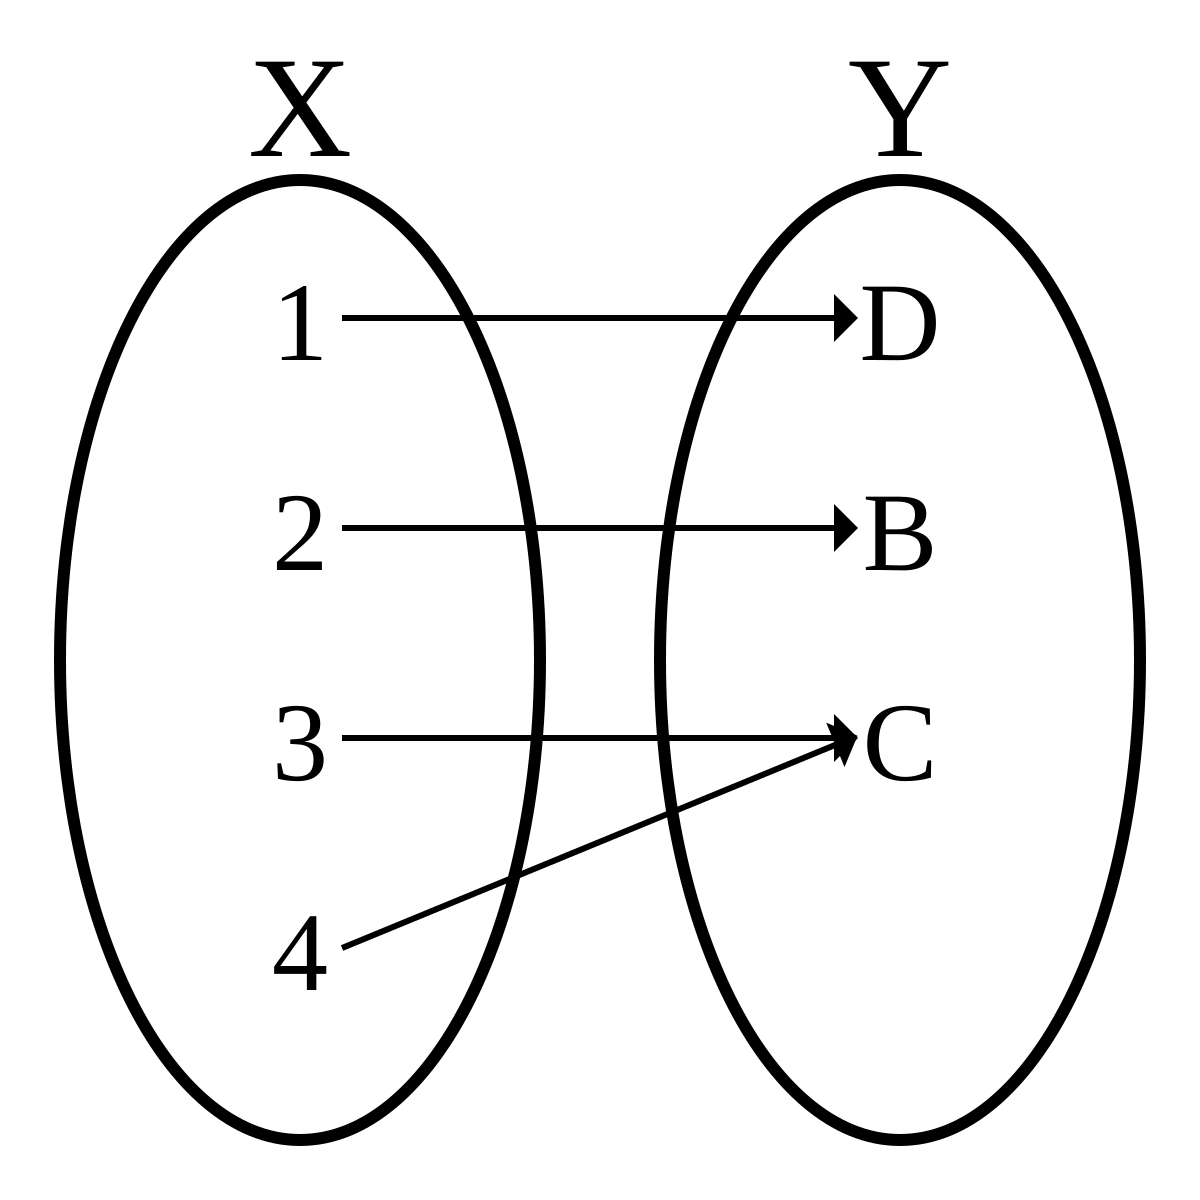
\includegraphics[width=.9\linewidth]{./src/surjection.png}
\end{center}
Отображение \(F \subset A \times B\) или \(F: A \rightarrow B\) называется сюръективным.
если \(\forall b \in B \exists a \in A: (a, b) \in F\).

Т.е. полностью покрывается все \(B\)

Например: Для каждой точки на плоскости есть треугольник с центром массы в ней.
\subsubsection{Вложение (инъекция)}
\label{sec:orgef00f20}
\begin{center}
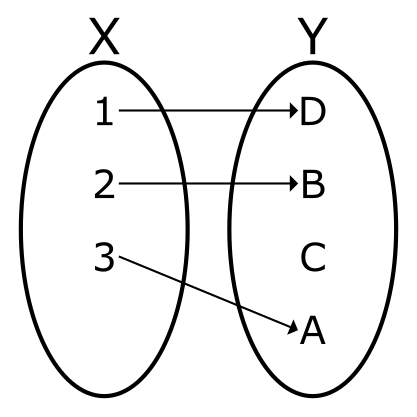
\includegraphics[width=.9\linewidth]{./src/Injection.png}
\end{center}
Отображение \(F \subset A \times B\) называется инъективным.
если \((a_1, b), (a_2, b) \in F \Rightarrow a_1 = a_2\).

Т.е. к каждому \(b\) соответсвует не больше 1 \(a\).

\(\forall b \in B: (\exists! a \in A: (a, b) \in F) \lor (\forall a \in A: (a, b) \notin F)\)
\subsubsection{Функция (обратная инъекция)}
\label{sec:org28f193e}
Отображени \(F \subset A \times B\) называется функцией, если
\((a_1, b_1), (a_1, b_2) \in F \Rightarrow b_1 = b_2\)

Т.е. к каждому \(a\) соответсвует не больше 1 \(a\)
\subsubsection{Область определения}
\label{sec:org3f0122b}
Областью определения \(F: A \rightarrow B\)
называется множество \(\text{dom} F = \{a \in A | \exists b \in B: (a, b) \in F\}\)

т.е. \(\exists b \in B: (a, b) \in F\) - предикат
\subsubsection{Область значений}
\label{sec:org7e60f97}
Областью значений \(F: A \rightarrow B\)
называется множество \(\text{rng} F = \{b \in B | \exists a \in A: (a, b) \in F\}\)
\subsubsection{Однозначность (биекция)}
\label{sec:org74f5851}
\begin{center}
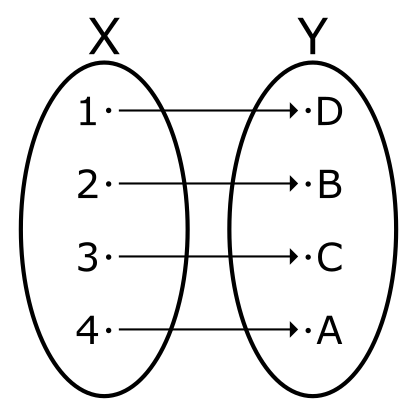
\includegraphics[width=.9\linewidth]{./src/Bijection.png}
\end{center}
Отображени \(F \subset A \times B\) называется биективным (1 к 1), если
\(F\) - сюръективно, инъективно, функция и \(\text{dom} F = A\)
\subsubsection{Вложение}
\label{sec:org2e138fb}
\(R \subset A \times B\) - вложене если \(R\) - функция, инъекция и \(\text{dom} R = A\)

Биекция - частный случай вложения.
\subsection{Обратное отображение}
\label{sec:orgc2e41ee}
Для отображения \(F: A \rightarrow B\) обратное отображение определяется как
\(F^{-1}: B \rightarrow A, F^{-1} = \{(b, a) | (a, b) \in F\}\) при \(F, F^{-1}\) сюръективных.
\subsubsection{Доказательство биекции}
\label{sec:org3c4e643}
\(F\) - биекция \(\iff F\) и \(F^{-1}\) сюръективные и функции

\(F^{-1}\) - функция \(\iff F\) - инъекция.

В сочетании с фактом того, что F\$ - сюръективная функция получается что \(F\) - биекция.
\section{Теорема Кантора - Бернштейна}
\label{sec:org21ffcdc}
Пусть \(A\) и \(B\) - множества.

\(\exists B_1 \subseteq B | F: A \rightarrow B_1\) - биекция

\(\exists A_1 \subseteq A | F: B \rightarrow A_1\) - биекция

Тогда \(A \textasciitilde B\)

Пока что без доказательства.
\end{document}
